\documentclass{standalone}
\usepackage{tikz}
\usepackage{amsmath}
\usepackage{color}

\usetikzlibrary{arrows.meta, calc, positioning, decorations.markings}

\begin{document}
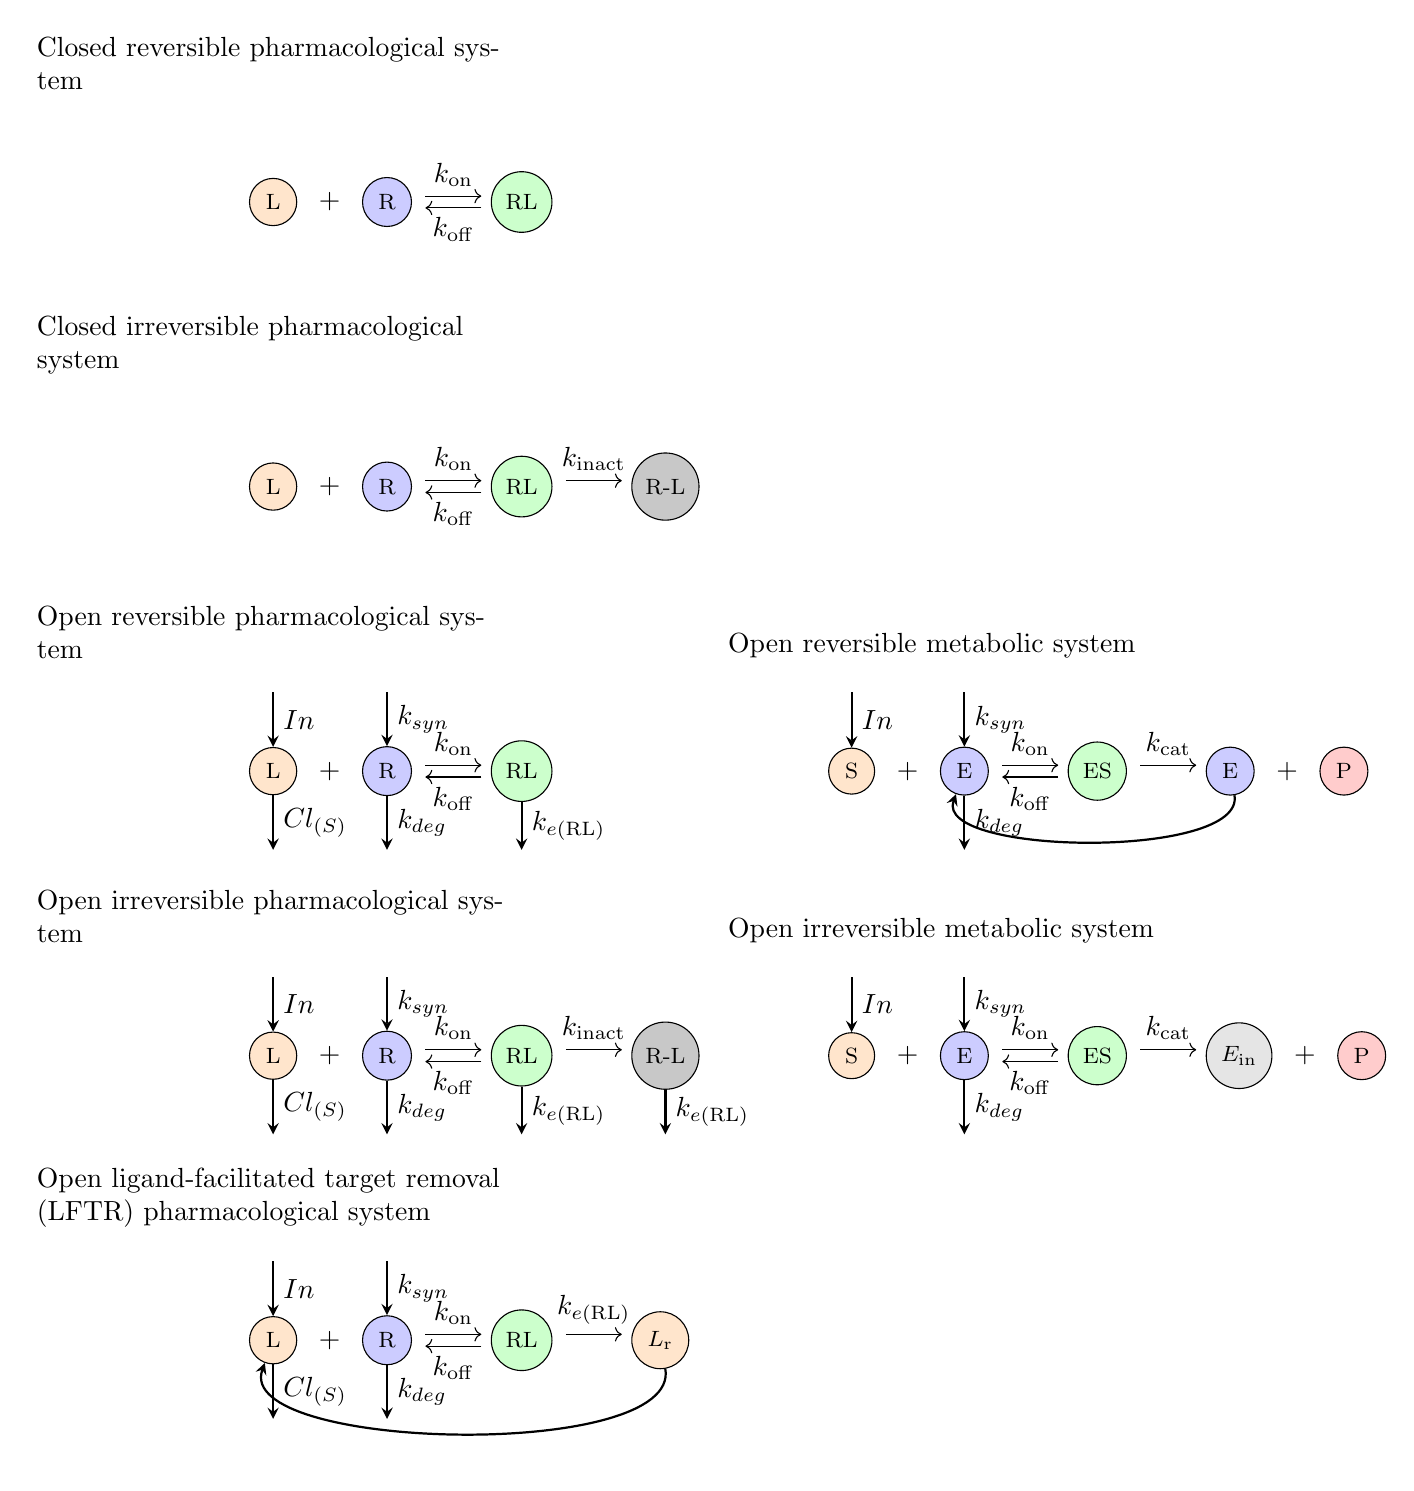
\begin{tikzpicture}[
    node distance=0.8cm,
    myoutarrow/.style={->, line width=0.8pt, >=stealth},
    myinarrow/.style={<-, line width=0.8pt, >=stealth},
    myleftarrow/.style={->, shorten >=2pt, shorten <=2pt},
    myrightarrow/.style={->, shorten >=2pt, shorten <=2pt},
    species/.style={circle, draw, font=\footnotesize, minimum size=1.2em, align=center},
    texts/.style={text width=6cm, align=left}
]

% define color
\definecolor{gray200}{RGB}{200,200,200}

% reaction 0: closed, reversible models

\node[species, fill=orange!20] (LC) {L};
\node[right=0.15cm of LC] (plusC) {$+$};
\node[species, fill=blue!20, right=0.15cm of plusC] (RC) {R};
\node[species, fill=green!20, right=1cm of RC] (RLC) {RL};

%--- Reversible arrows with k_on / k_off
\draw[myleftarrow]
  ($(RC.east)+(0.1,0.075)$) -- 
  node[above] {$k_{\mathrm{on}}$}
  ($(RLC.west)+(-0.05,0.075)$);

\draw[myrightarrow]
  ($(RLC.west)+(-0.05,-0.075)$) -- 
  node[below] {$k_{\mathrm{off}}$}
  ($(RC.east)+(0.1,-0.075)$);

% reaction 0r: closed, irreversible (e.g. covalent) system
\node[species, fill=orange!20, below=3cm of LC] (LCI) {L};
\node[right=0.15cm of LCI] (plusCI) {$+$};
\node[species, fill=blue!20, right=0.15cm of plusCI] (RCI) {R};
\node[species, fill=green!20, right=1cm of RCI] (RLCI) {RL};
\node[species, fill=gray200, right=1cm of RLCI] (inactRLCI) {R-L};

\draw[myleftarrow]
  ($(RCI.east)+(0.1,0.075)$) -- 
  node[above] {$k_{\mathrm{on}}$}
  ($(RLCI.west)+(-0.05,0.075)$);

\draw[myrightarrow]
  ($(RLCI.west)+(-0.05,-0.075)$) -- 
  node[below] {$k_{\mathrm{off}}$}
  ($(RCI.east)+(0.1,-0.075)$);

\draw[myleftarrow]
  ($(RLCI.east)+(0.1,0.075)$) -- 
  node[above] {$k_{\mathrm{inact}}$}
  ($(inactRLCI.west)+(-0.05,0.075)$);

% reaction 1: open, reversible systems
\node[species, fill=orange!20, below=3cm of LCI] (L) {L};
\node[right=0.15cm of L] (plus) {$+$};
\node[species, fill=blue!20, right=0.15cm of plus] (R) {R};
\node[species, fill=green!20, right=1cm of R] (RL) {RL};

%--- Reversible arrows with k_on / k_off
\draw[myleftarrow]
  ($(R.east)+(0.1,0.075)$) -- 
  node[above] {$k_{\mathrm{on}}$}
  ($(RL.west)+(-0.05,0.075)$);

\draw[myrightarrow]
  ($(RL.west)+(-0.05,-0.075)$) -- 
  node[below] {$k_{\mathrm{off}}$}
  ($(R.east)+(0.1,-0.075)$);

\draw[myinarrow] (L) -- node[right] {$In$} ++(0, 1);
\draw[myoutarrow] (L) -- node[right] {$Cl_{(S)}$} ++(0,-1);
\draw[myinarrow] (R) -- node[right] {$k_{syn}$} ++(0, 1);
\draw[myoutarrow] (R) -- node[right] {$k_{deg}$} ++(0,-1);
\draw[myoutarrow] (RL) -- node[right] {$k_{e\text{(RL)}}$} ++(0,-1);

% reaction 2: open, irreversible systems
\node[species, fill=orange!20, below=3cm of L] (L2) {L};
\node[right=0.15cm of L2] (plus2) {$+$};
\node[species, fill=blue!20, right=0.15cm of plus2] (R2) {R};
\node[species, fill=green!20, right=1cm of R2] (RL2) {RL};
\node[species, fill=gray200, right=1cm of RL2] (RL2I) {R-L};

\draw[myleftarrow]
  ($(R2.east)+(0.1,0.075)$) -- 
  node[above] {$k_{\mathrm{on}}$}
  ($(RL2.west)+(-0.05,0.075)$);
\draw[myrightarrow]
  ($(RL2.west)+(-0.05,-0.075)$) -- 
  node[below] {$k_{\mathrm{off}}$}
  ($(R2.east)+(0.1,-0.075)$);
\draw[myleftarrow]
  ($(RL2.east)+(0.1,0.075)$) -- 
  node[above] {$k_{\mathrm{inact}}$}
  ($(RL2I.west)+(-0.05,0.075)$);

\draw[myinarrow] (L2) -- node[right] {$In$} ++(0, 1);
\draw[myoutarrow] (L2) -- node[right] {$Cl_{(S)}$} ++(0,-1);
\draw[myinarrow] (R2) -- node[right] {$k_{syn}$} ++(0, 1);
\draw[myoutarrow] (R2) -- node[right] {$k_{deg}$} ++(0,-1);
\draw[myoutarrow] (RL2) -- node[right] {$k_{e\text{(RL)}}$} ++(0,-1);
\draw[myoutarrow] (RL2I) -- node[right] {$k_{e\text{(RL)}}$} ++(0,-1);

% reaction 3: Ligand-facilitated target removal
\node[species, fill=orange!20, below=3cm of L2] (L3) {L};
\node[right=0.15cm of L3] (plus3) {$+$};
\node[species, fill=blue!20, right=0.15cm of plus3] (R3) {R};
\node[species, fill=green!20, right=1cm of R3] (RL3) {RL};
\node[species, fill=orange!20, right=1cm of RL3] (L3r) {$L_{\text{r}}$};

\draw[myleftarrow]
  ($(R3.east)+(0.1,0.075)$) -- 
  node[above] {$k_{\mathrm{on}}$}
  ($(RL3.west)+(-0.05,0.075)$);
\draw[myrightarrow]
  ($(RL3.west)+(-0.05,-0.075)$) -- 
  node[below] {$k_{\mathrm{off}}$}
  ($(R3.east)+(0.1,-0.075)$);
\draw[myrightarrow]
  ($(RL3.east)+(0.1,0.075)$) -- 
  node[above] {$k_{e\text{(RL)}}$}
  ($(L3r.west)+(-0.05,0.075)$);

\draw[myinarrow] (L3) -- node[right] {$In$} ++(0, 1);
\draw[myoutarrow] (L3) -- node[right] {$Cl_{(S)}$} ++(0,-1);
\draw[myinarrow] (R3) -- node[right] {$k_{syn}$} ++(0, 1);
\draw[myoutarrow] (R3) -- node[right] {$k_{deg}$} ++(0,-1);

\draw[myoutarrow] (L3r) to[out=-80,in=-110,looseness=0.6] (L3);

% reaction 4: Reversible metabolic system
\node[species, fill=orange!20, right=3.5cm of RL] (S) {S};
\node[right=0.15cm of S] (plus4) {$+$};
\node[species, fill=blue!20, right=0.15cm of plus4] (E) {E};
\node[species, fill=green!20, right=1cm of E] (ES) {ES};
\node[species, fill=blue!20, right=1cm of ES] (Er) {E};
\node[right=0.15cm of Er] (plus4r) {$+$};
\node[species, fill=red!20, right=0.15cm of plus4r] (P) {P};

\draw[myleftarrow]
  ($(E.east)+(0.1,0.075)$) -- 
  node[above] {$k_{\mathrm{on}}$}
  ($(ES.west)+(-0.05,0.075)$);
\draw[myrightarrow]
  ($(ES.west)+(-0.05,-0.075)$) -- 
  node[below] {$k_{\mathrm{off}}$}
  ($(E.east)+(0.1,-0.075)$);
\draw[myleftarrow]
  ($(ES.east)+(0.1,0.075)$) -- 
  node[above] {$k_{\mathrm{cat}}$}
  ($(Er.west)+(-0.05,0.075)$);

\draw[myinarrow] (S) -- node[right] {$In$} ++(0, 1);
\draw[myinarrow] (E) -- node[right] {$k_{syn}$} ++(0, 1);
\draw[myoutarrow] (E) -- node[right] {$k_{deg}$} ++(0,-1);
\draw[myoutarrow] (Er) to[out=-80,in=-110,looseness=0.6] (E);

% reaction 5: irreversible metabolic system
\node[species, fill=orange!20, right=3.5cm of RL2] (S2) {S};
\node[right=0.15cm of S2] (plus5) {$+$};
\node[species, fill=blue!20, right=0.15cm of plus5] (E2) {E};
\node[species, fill=green!20, right=1cm of E2] (ES2) {ES};
\node[species, fill=gray!20, right=1cm of ES2] (Einact) {$E_{\mathrm{in}}$};
\node[right=0.15cm of Einact] (plus5r) {$+$};
\node[species, fill=red!20, right=0.15cm of plus5r] (P2) {P};

\draw[myleftarrow]
  ($(E2.east)+(0.1,0.075)$) -- 
  node[above] {$k_{\mathrm{on}}$}
  ($(ES2.west)+(-0.05,0.075)$);
\draw[myrightarrow]
  ($(ES2.west)+(-0.05,-0.075)$) -- 
  node[below] {$k_{\mathrm{off}}$}
  ($(E2.east)+(0.1,-0.075)$);
\draw[myleftarrow]
  ($(ES2.east)+(0.1,0.075)$) -- 
  node[above] {$k_{\mathrm{cat}}$}
  ($(Einact.west)+(-0.05,0.075)$);

\draw[myinarrow] (S2) -- node[right] {$In$} ++(0, 1);
\draw[myinarrow] (E2) -- node[right] {$k_{syn}$} ++(0, 1);
\draw[myoutarrow] (E2) -- node[right] {$k_{deg}$} ++(0,-1);




% text annotations
\node[texts, above=1.0cm of LC] {Closed reversible pharmacological system};
\node[texts, above=1.0cm of LCI] {Closed irreversible pharmacological system};
\node[texts, above=1.0cm of L] {Open reversible pharmacological system};
\node[texts, above=1.0cm of L2] {Open irreversible pharmacological system};
\node[texts, above=1.0cm of L3] {Open ligand-facilitated target removal (LFTR) pharmacological system};
\node[texts, above=1.0cm of E] {Open reversible metabolic system};
\node[texts, above=1.0cm of E2] {Open irreversible metabolic system};

\end{tikzpicture}
\end{document}
